\section{Effets :}
\textbf{NB:} Tous les effets nécessitant un histogramme utilise celui de la "\emph{valeur}", soit le maximum entre les trois canaux de l'espace de couleur Rouge Vert Bleu.

\subsection{Luminosité (Brightness) :}
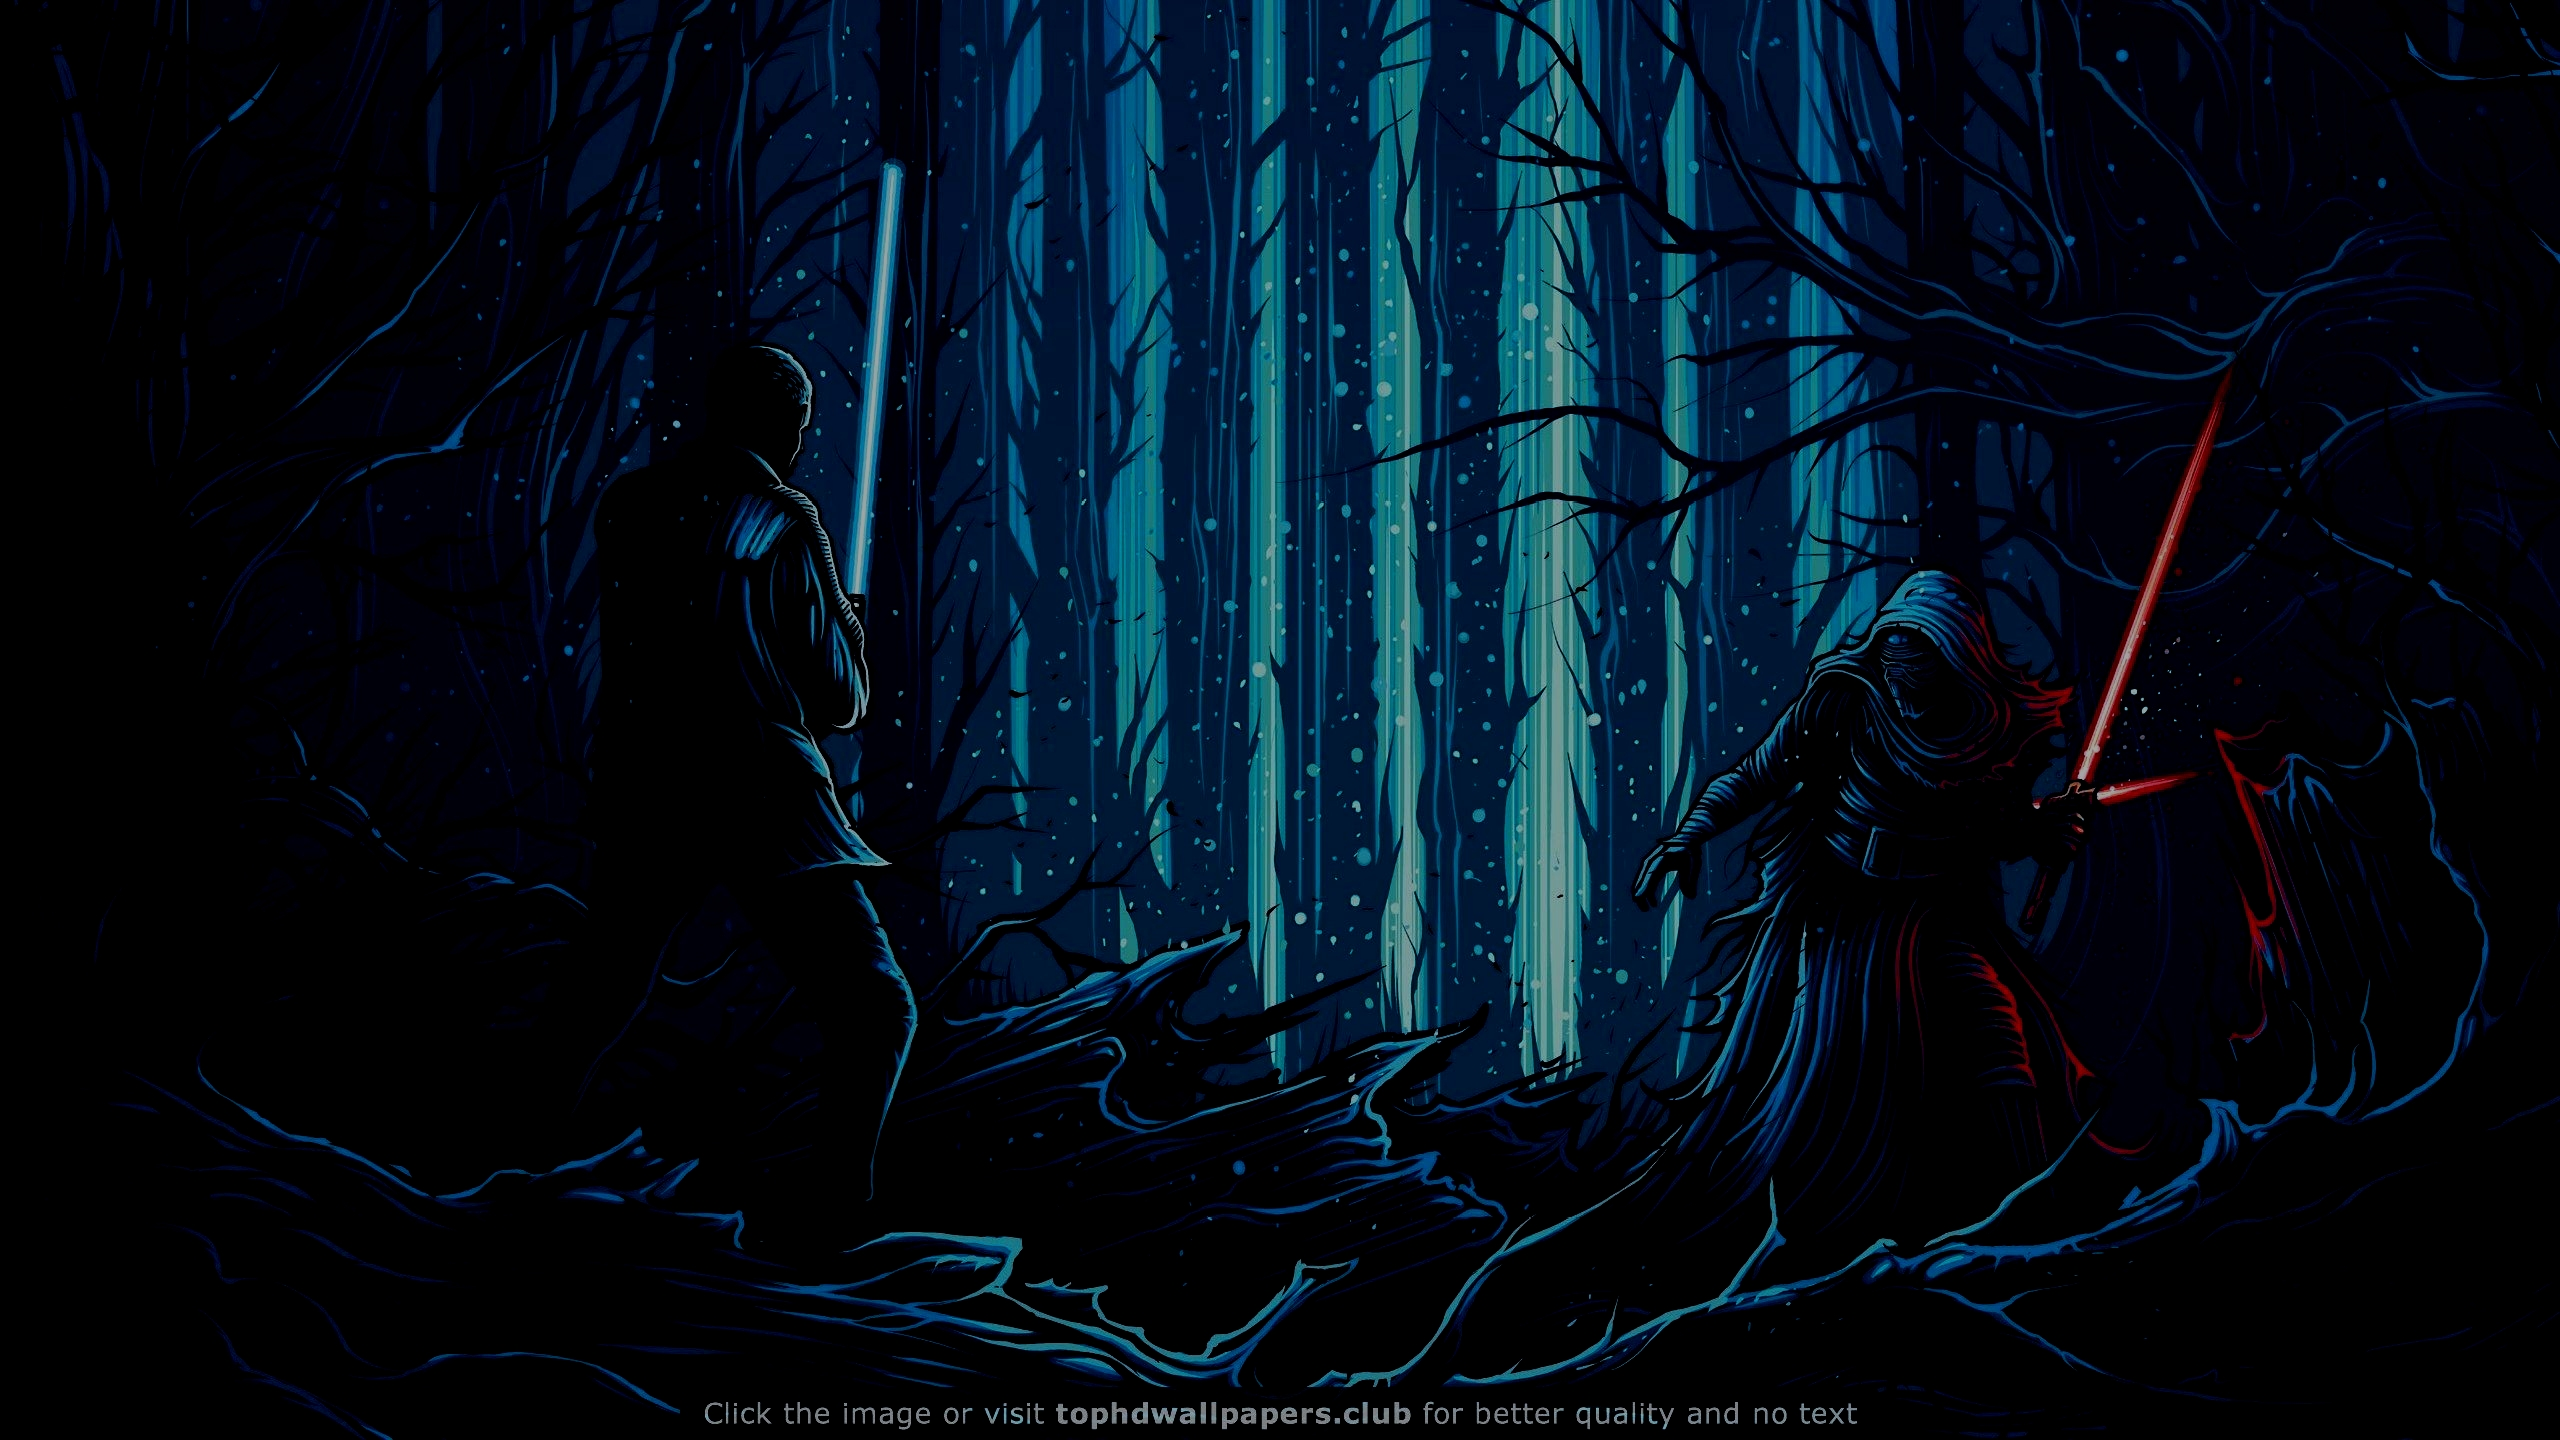
\includegraphics[width=0.5\textwidth]{report_src/brightness_low.jpeg}
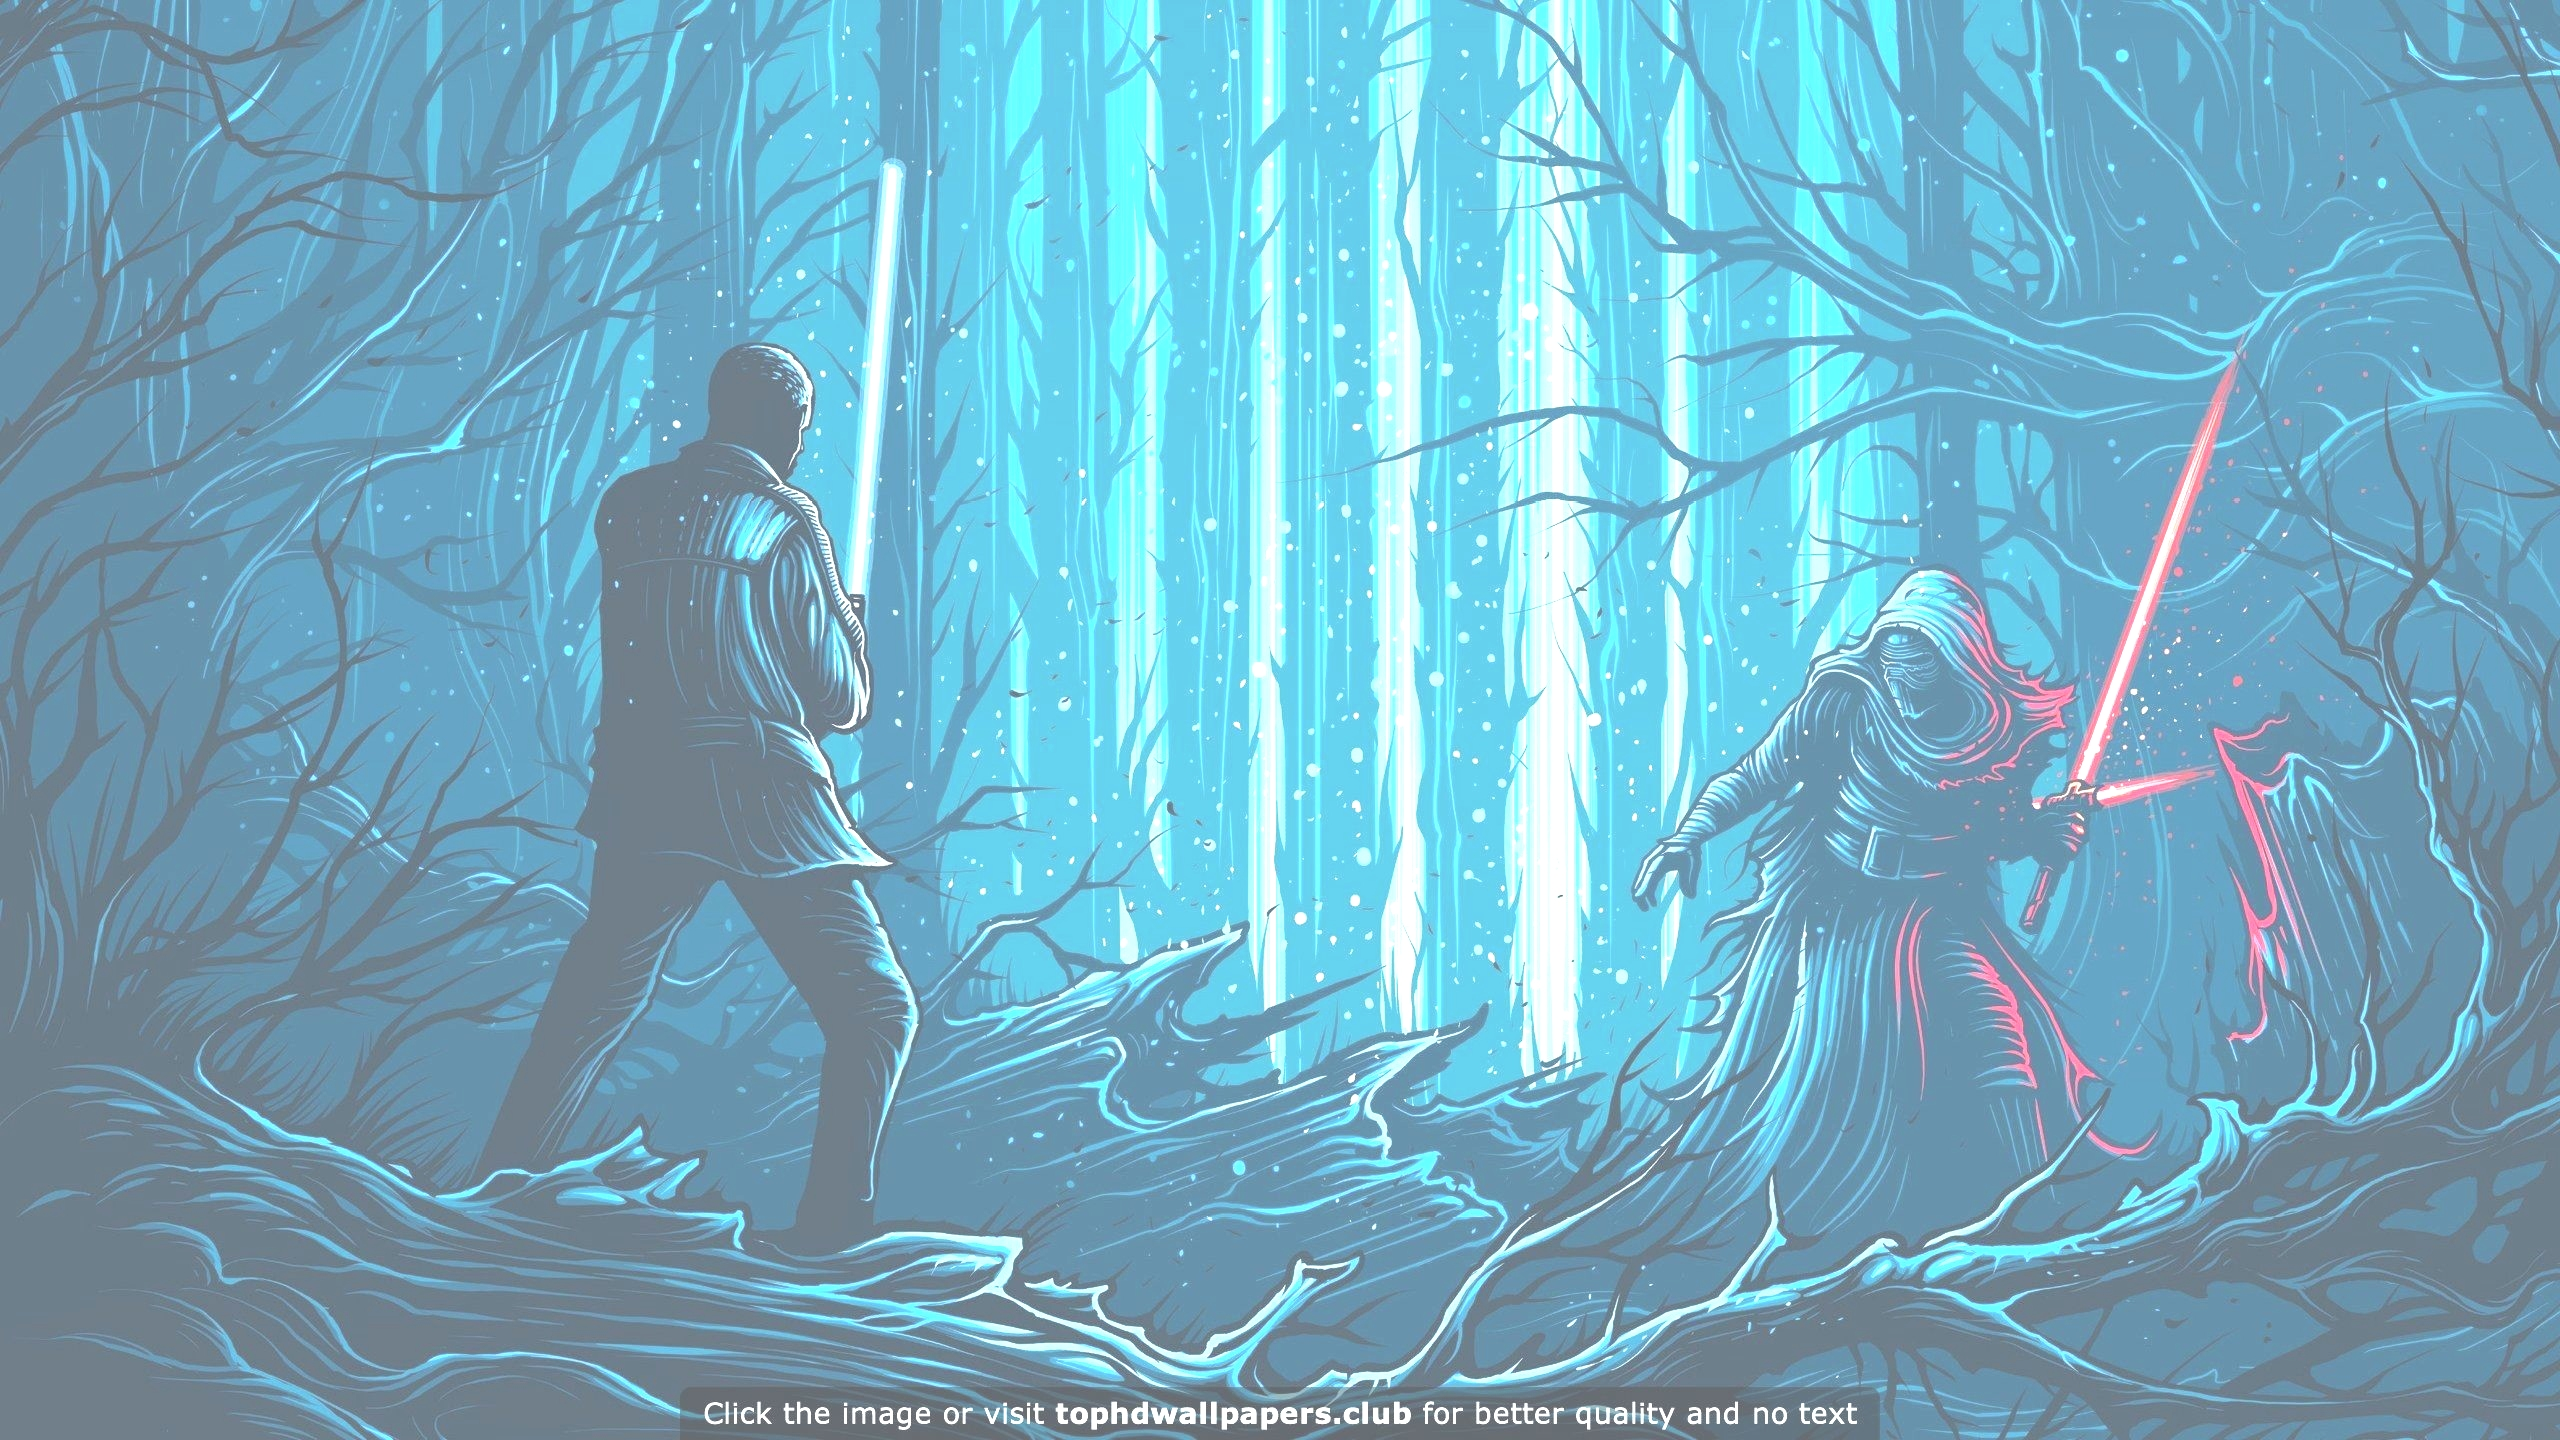
\includegraphics[width=0.5\textwidth]{report_src/brightness_high.jpeg}

\emph{Méthode appelante : Retouching.setBrightness()}

\emph{Script : brightness.rs}
\\

Ce réglage ajoute une valeur (positive ou négative) aux trois canaux RGB de l'image. Cette valeur est fixée par la seekbar.
Les valeurs sont tronquées entre 0 et 255, par conséquent on perd de l'information dans les valeurs extrêmes de luminosité.

Cet effet n'utilise pas la luminosité existante de l'image, ainsi on peut obtenir des résultats qui sont parfois discutables, par exemple
le noir qui s'éclaircit et inversement pour le blanc. Pour pallier à ce problème, on pourrait introduire une multiplication afin de modifier
la luminosité proportionnellement à celle existante. Cependant, cette solution modifie aussi le contraste, nous avons donc choisi
de laisser l'algorithme tel quel.


\subsection{Contraste (Contrast) :}

\emph{Méthode appelante : Retouching.dynamicExtensionRGB()}

\emph{Script : dynamicExtension.rs}
\\

Ce réglage effectue une extension linéaire de dynamique. Les nouveaux extremum de l'histogramme sont définis à partir de la position de la seekbar.
La dynamique est ainsi étendue autour d'une valeur se situant au milieu des deux anciens extremum de l'histogramme*. On a donc une image uniforme lorsque
l'on règle le contraste au minimum. En augmentant le contraste, les extremum peuvent sortir de l'intervalle [0;255], ce qui provoque une distorsion de l'image.
\\

*Il serait peut-être plus judicieux de prendre la médiane de l'histogramme cumulé afin d'avoir une valeur qui représente mieux la "valeur moyenne" de l'image.


\subsection{Saturation (Saturation) :}

\emph{Méthode appelante : Retouching.setSaturation()}

\emph{Script : saturation.rs}
\\

Ce réglage permet de régler la saturation de l'image. Soit S la saturation existante, S' la nouvelle saturation et F le facteur de saturation. S et S' vont de 0 à 1.

On a S' = S + F * (1 - S) * S. 

On observe que la nouvelle saturation est proportionnelle à deux facteurs : l'espace restant avant une saturation totale (1-S) et la saturation existante S.
Par conséquent, en augmentant la saturation, chaque pixel tend vers sa saturation maximale, tout en garantissant une saturation proportionnelle à celle existante, évitant ainsi de saturer le gris.

\subsection{Egalisation d'histogramme (Enhance) :}

\emph{Méthode appelante : Retouching.histogramEqualization()}

\emph{Scripts : cumulativeHistogram.rs, assignLut.rs} 
\\

Comme son nom l'indique, cet effet utilise l'égalisation d'histogramme afin d'améliorer le contraste.
On calcule d'abord l'histogramme cumulé et on en déduit la LUT (Look Up Table), que nous assignons ensuite à chaque pixel.
\\

Cependant, afin d'égaliser l'histogramme, l'algorithme éclaircit les zones sombres, ce qui donne un résultat peu convaincant sur les images de faible luminosité.
Une solution à ce problème est l'égalisation d'histogramme adaptative (CLAHE), mais nous n'avons pas eu le temps de l'implémenter pour ce rendu.

\subsection{Convolution (Blur, Sharpen, Neon) :}

    Dans cette sous-section on retrouve des effets réalisés avec des convolutions pour flouter une image en passant par deux types différents de kernel : Gaussien et moyenneur
    (bouton "Blur"), des effets pour améliorer la netteté d'une image avec la fonction "Laplacian of gaussian" (bouton Sharpen) et des effets de 
    détection de contours (bouton "Neon") en réalisant des convolutions avec des opérateurs comme Sobel, Prewitt, Kirsch ou une convolution simple avec un kernel
    laplacien.
    \\

    Pour ces effets nous avons implémenté 3 méthodes de convolution.


    \begin{itemize}
        \item Convolution classique.
        \item Convolution séparable.
        \item Convolution détection de contours.
    \end{itemize}
    

    \subsubsection*{Convolution classique}
    
        Cette méthode de convolution suit le même algorithme vu en cours, on peut l'appliquer avec des noyaux asymétriques de dimensions impaires uniquement,
        cette opération a été parallélisée grâce à l'outil "renderscript" qui parallélise le calcul par CPU multithreading/GPU. En plus dans cette méthode (et dans toutes les autres) nous avons rajouté
        des optimisations pour parcourir seulement les index nécessaires de l'image lors de la convolution. En calculant les index des centres des deux dimensions du kernel
        on peut anticiper et éviter les appels de fonction inutiles sur les bords de l'image par exemple.
        
        $X_{d\acute{e}but}$ et $X{fin}$ étant le premier et dernier index à parcourir dans l'axe des abscisses respectivement et
        $Y_{d\acute{e}but}$ et $Y_{fin}$ étant le premier et dernier index à parcourir dans l'axe des ordonnées respectivement.
        \[
            Kernel_{CentreX} =   \frac{Largeur_{kernel}}{2}            
        \]
        \[
            Kernel_{CentreY} =   \frac{Hauteur_{kernel}}{2}            
        \]
        \[
            X_{d\acute{e}but} = Kernel_{CentreX}      
        \]
        \[
            X_{fin} = Largeur_{image} - Kernel_{CentreX}           
        \]
        \[
            Y_{d\acute{e}but} = Kernel_{CentreY}      
        \]
        \[
            Y_{fin} = Hauteur_{image} - Kernel_{CentreY}           
        \]

        En définissant les index du début et de fin de parcours pour les deux dimensions de l'image sur le script de lancement renderscript
        comme ci-dessus on peut s'en passer de quelques appels de fonctions sur les bords de l'image et ainsi gagner du temps de calcul.

    \subsubsection*{Convolution séparable}

        Pour la convolution classique avec un kernel de taille $N*M$ on doit faire $N*M$ multiplications pour chaque échantillon,
        cependant si le kernel est séparable on peut passer à $N+M$ opérations.
        \\

        Or afin d'optimiser le calcul de la convolution sur des filtres séparables comme le filtre gaussien et moyenneur nous avons implémenté une
        méthode de convolution séparable.
        
        \begin{figure}[!h]
            \centering
            \begin{subfigure}[b]{1\textwidth}
                \centering
                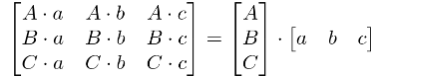
\includegraphics[width=0.5\textwidth]{report_src/separableConv1.png}
            \end{subfigure}
        \end{figure}

        Un kernel est séparable quand sa matrice des poids peut être représentée par le produit de deux vecteurs.
        \\

        Ce calcul est réalisé en faisant deux convolutions unidimensionnelles successives (en X et en Y) sur l'image d'origine en stockant le résultat dans une image intermédiaire.
        La propriété d'associativité de la convolution rend ce calcul possible.

        \[
            x * (N * N)  \iff (x * N) * N
        \]

        La limite de cette méthode c'est que l'on doit passer par une image partielle pour la réalisation du calcul en
        utilisant plus de mémoire que pour une convolution classique.



    \subsubsection*{Convolution détection de contours}

        Cette méthode prend en paramètre deux kernels de même taille et réalise deux convolutions avec chaque kernel et ensuite calcule le produit des deux.
        Vu que ces deux convolutions sont indépendantes l'une de l'autre on peut se permettre de les réaliser au même temps dans le script et de faire l'addition
        des valeurs absolues résultantes des deux accumulateurs. Comme son nom l'indique cette méthode est utilisée notamment pour faire des convolutions pour la détection de contours
        avec des opérateurs comme Sobel, Kirsch, Prewitt, etc.
    \\

    Un des points de réflexion sur la convolution c'est que jusqu'à présent on la réalise sur les 3 canaux RGB, ce qui est assez lourd au niveau de calcul,
    cependant on pourrait passer l'image en échelle de gris et la faire seulement sur un des canaux ou passer pour l'espace HSV en utilisant la value ou la saturation.
    \newpage

    \subsubsection*{Les kernels} \label{kernels}

    Tous les kernels sont définis dans la classe fr.ubordeaux.pimp.util.Kernels. Les kernels de détection de contour (Sobel, Kirsch, Laplace, Prewitt) sont définis
    en variable statique et finale, car leur taille est fixe, les autres sont générés par une méthode. Si on prend le cas du kernel de Gauss, la méthode gauss permet 
    de générer la version séparée du kernel, c'est-à-dire une seule ligne. Les méthodes génératrices de kernel prennent en argument la taille de celui-ci, ce qui sert
    aux effets paramétrables tels que blur et sharpen.

    \subsubsection{Flou gaussien et moyenneur (Blur) : }

        \begin{figure}[!h]
            \centering
            \begin{subfigure}[b]{0.4\textwidth}
                \includegraphics[width=1\textwidth]{report_src/picOrg.jpeg}
            \end{subfigure}
            \begin{subfigure}[b]{0.4\textwidth}
                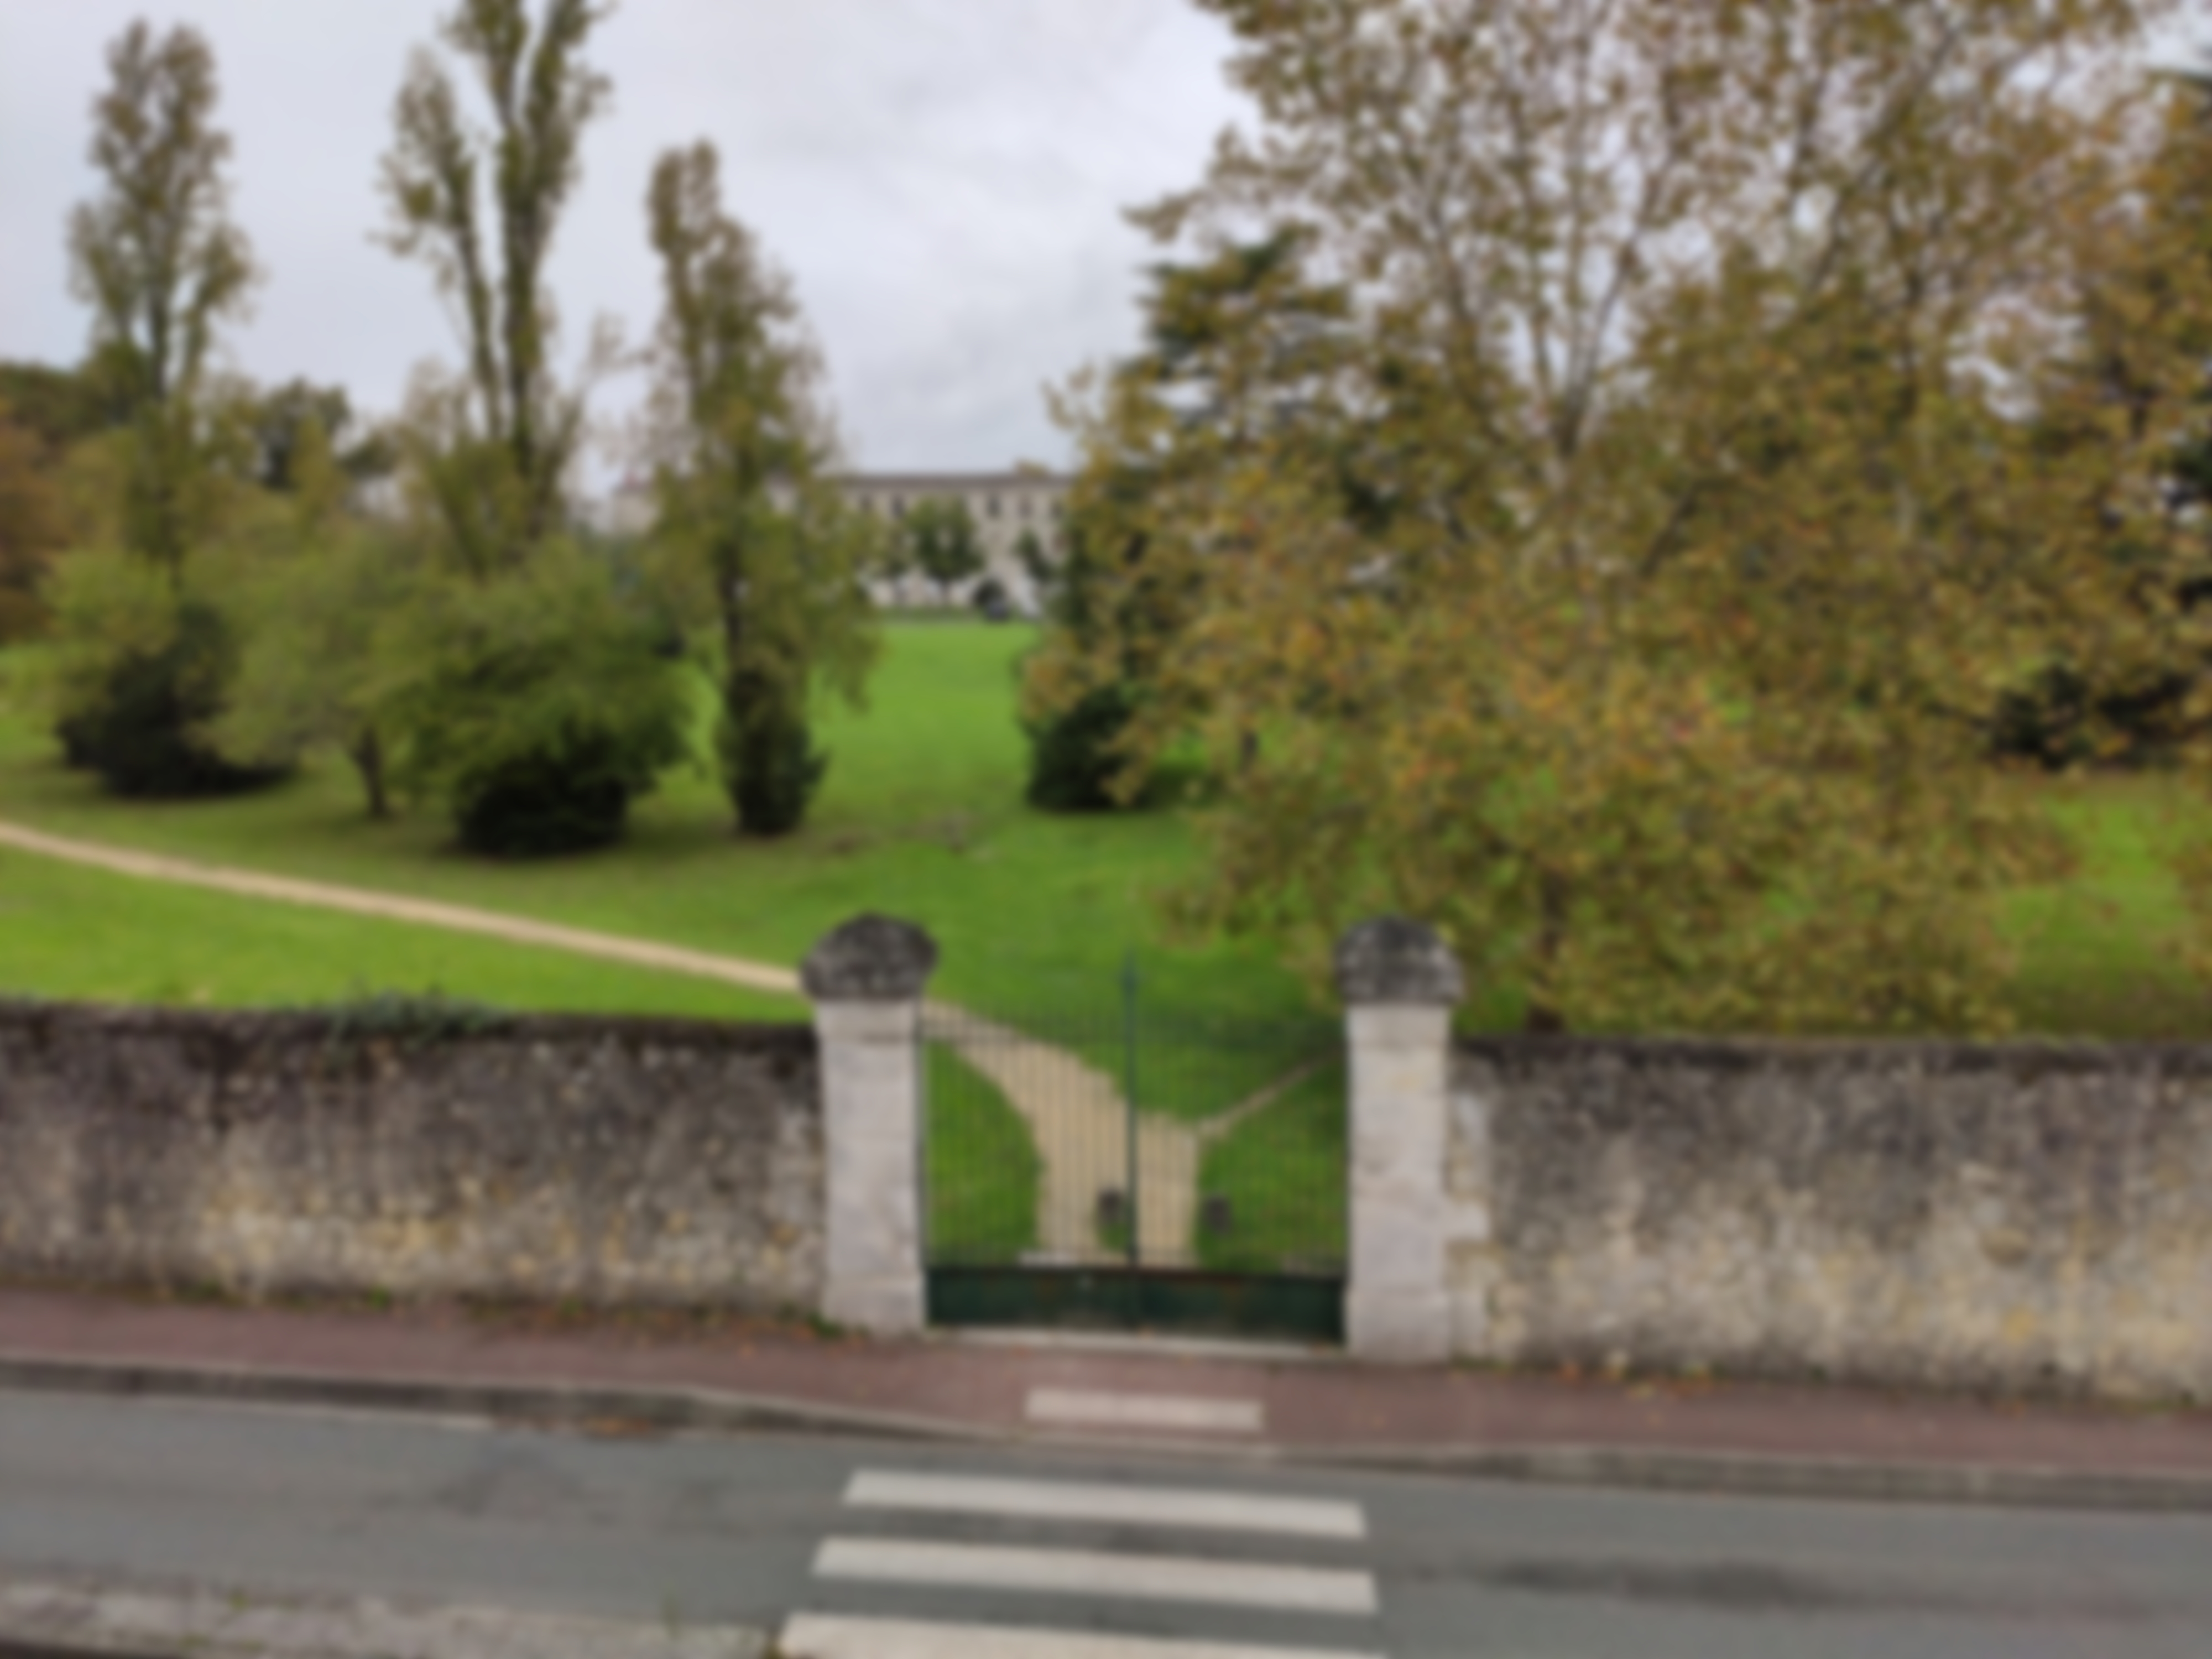
\includegraphics[width=1\textwidth]{report_src/blur.jpeg}
            \end{subfigure}
        \end{figure} 
        \emph{Méthode appelante : Convolution.gaussianBlur()}

        \emph{Scripts : convolution.rs} 





        
